\documentclass{ctexart} 
\title{整本书公式整理}
\author{欧 宇恒}
\date{\today}
\usepackage{ctex}			%处理中文字体宏包
\usepackage{graphicx}		%处理图片宏包
\usepackage{amsmath}		%处理数学公式宏包	
\usepackage{setspace}		%处理行距宏包
\usepackage[left=1.91cm,right=1.91cm,top=2.54cm,bottom=2.54cm]{geometry}		%编辑页面格式
\usepackage{booktabs}		%处理三线表宏包
\usepackage{color}			%处理颜色宏包
%\begin{处理页眉页脚}
\usepackage[english]{babel}
\usepackage[utf8]{inputenc}
\usepackage{fancyhdr}

\pagestyle{fancy}
\fancyhf{}
\rhead{\kaishu \leftmark}
\lhead{\kaishu 交通院辅学——大物公式整理}
\rfoot{Page \thepage}
%\end{处理页眉页脚}


\begin{document}	
	\ctexset{
		section={
			name={\S},
			nameformat={\color{cyan}\zihao{4}\bfseries},
			titleformat={\color{cyan}\centering\heiti\zihao{4}},
		},
		subsection={
			name={},
			nameformat={\color{cyan}\zihao{4}\bfseries},
			titleformat={\color{cyan}\kaishu\zihao{4}},
		},
	}
%%封面
\begin{center}

\includegraphics[scale=0.6]{images//logo.png} 

	\begin{spacing}{2.0}
		\kaishu \zihao{-0}{大学物理公式整理}
	\end{spacing}

	\begin{spacing}{1.5}
		\LARGE

		\begin{tabular}{r l}
		编辑& 欧宇恒\\
		\end{tabular}

		date: \today

		本文档仅作为公式整理,并不能作为知识清单的知识点汇总使用
	\end{spacing}
\end{center}

\newpage

\tableofcontents

\newpage

\section{静电场}

\subsection{库仑定律与若干带电系统电场与电势大小}

$$F=\frac{1}{4\pi \varepsilon_0}\frac{q_1q_2}{r^2}$$

表征两点电荷之间的静电力

电场的定义式:

$$\vec{E}=\frac{\Sigma \vec{F}}{q}$$



\subsubsection{电偶极子电场大小}

\begin{figure}[h]
	\centering
	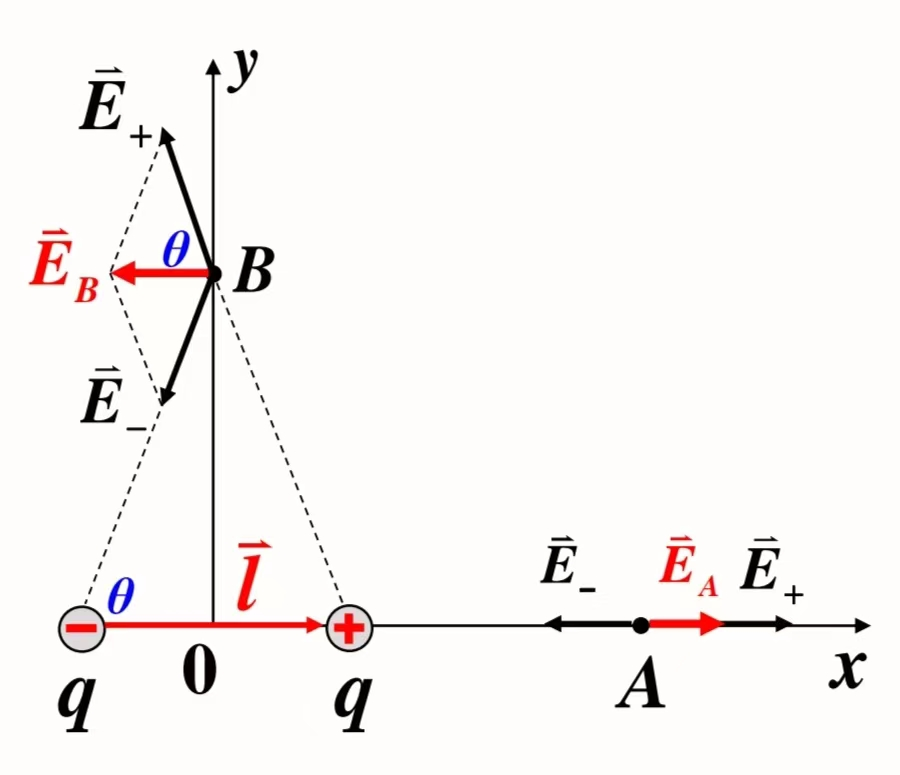
\includegraphics[scale=0.2]{images//chapter_10//figure_10.1.jpg} 
	\caption{电偶极子示意图}\label{figure1}
\end{figure}

A处场强——

$$\vec{E_A}=\frac{1}{4\pi \varepsilon_0}\frac{2\vec{p}}{r^3}$$

B处场强——

$$\vec{E_B}=-\frac{1}{4\pi \varepsilon_0}\frac{\vec{p}}{r^3}$$

其中,$\vec{p}=q\vec{l}$,由负电荷指向正电荷;

只需要记结论,不需要记推导(太复杂啦)

\subsubsection{均匀带电细直棒外任意一点场强大小}

(如图\ref{figure2}所示)

\begin{figure}[h]
	\centering
	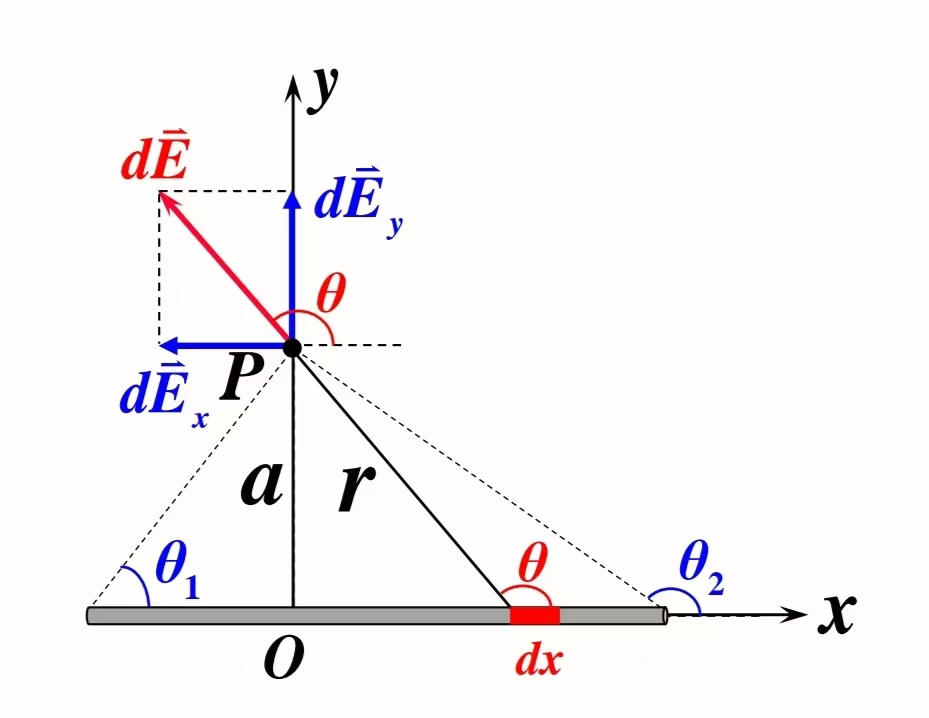
\includegraphics[scale=0.2]{images//chapter_10//figure_10.2.jpg} 
	\caption{均匀带电细直棒外任意一点场强}\label{figure2}
\end{figure}

$$E_x=\frac{\lambda}{4\pi \varepsilon_0a}(\sin\theta_2-\sin\theta_1)$$

$$E_y=\frac{\lambda}{4\pi \varepsilon_0a}(\cos\theta_1-\cos\theta_2)$$

(注意$\theta_1$和$\theta_2$的位置顺序不同,了解即可,不必硬记)

\textbf{对于无限长均匀带电细直棒}

$$E=\frac{\lambda}{2\pi \varepsilon_0a}$$

若$\lambda >0$,则$\vec{E}$垂直细棒向外;
若$\lambda <0$,则$\vec{E}$垂直细棒向内;

\subsubsection{均匀带电圆环轴线上距环心$x$处的电场与电势大小}

(如图\ref{figure3}所示)

\begin{figure}[h]
	\centering
	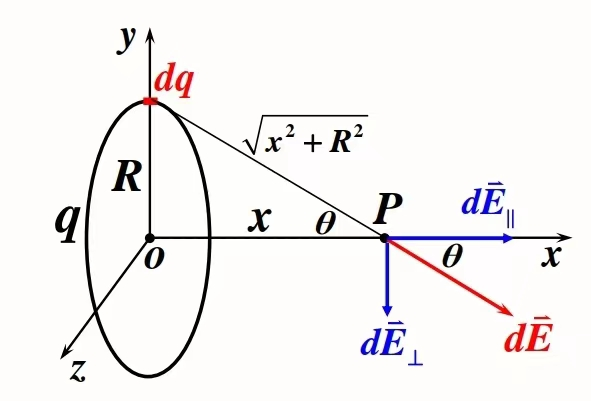
\includegraphics[scale=0.4]{images//chapter_10//figure_10.3.jpg} 
	\caption{均匀带电圆环轴线上距环心$x$处的电场}\label{figure3}
\end{figure}

$$\vec{E}=\frac{xq}{4\pi \varepsilon_0 (R^2+x^2)^{\frac{3}{2}}}\vec{i}$$

场强沿轴线方向

电势大小:

$$\varphi=\frac{q}{4\pi \varepsilon_0\sqrt{R^2+x^2}}$$


\subsubsection{无限大均匀带电平面的场强大小}

(如图\ref{figure4}所示)

\begin{figure}[h]
	\centering
	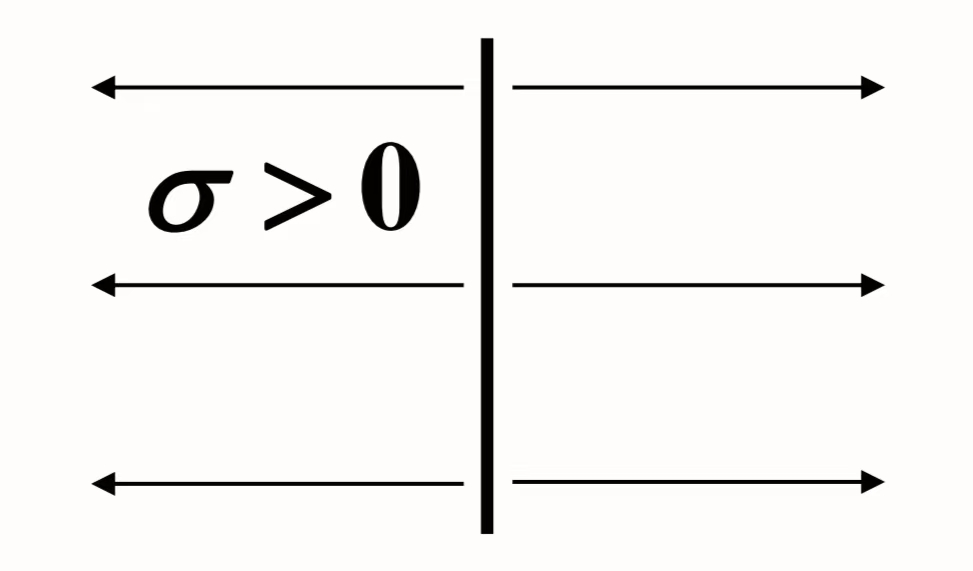
\includegraphics[scale=0.2]{images//chapter_10//figure_10.4.jpg} 
	\caption{无限大均匀带电平面的场强}\label{figure4}
\end{figure}

$$E=\frac{\sigma}{2\varepsilon_0}$$

\subsubsection{均匀带电球面的电势分布}

\begin{equation*}
\vec{E}=
	\begin{cases}
\frac{q}{4\pi \varepsilon_0R},&r<R\\
\frac{q}{4\pi \varepsilon_0r},&r>R\\
\end{cases}
\end{equation*}

\subsection{高斯定理}

$$\oint_{S}\vec{E}\cdot d\vec{S}=\frac{\Sigma q_i}{\varepsilon_0}$$

(由于本文档仅做公式整理,故不展开公式的具体运用,下同)

\subsection{静电场的环路定理}

$$\oint_{L}\vec{E}\cdot d\vec{l}=0$$

\subsection{电势能}

$$W_a=\int_{a}^{\infty}q_0\vec{E}\cdot d\vec{l}$$

$q_0$在静电场中$a$点的电势能,等于将$q_0$从$a$点移到电势能零点,静电力所做的功

\subsection{电势}

$$\varphi_a=\frac{W_a}{q}=\int_{a}^{\infty}\vec{E}\cdot d\vec{l}$$

电势叠加原理:代数加和$\varphi=\int d\varphi$

\section{静电场中的导体与电介质}

\subsection{导体表面附近的场强}

$$\vec{E}=\frac{\sigma}{\varepsilon_0}$$

方向与导体垂直

\subsection{电场与电势计算总结}

\begin{equation*}
\text{计算}\vec{E}\begin{cases}
	\text{1.定义}&\vec{E}=\frac{\vec{F}}{q_0} 
	\rightarrow \text{点电荷} \rightarrow 
	\vec{E}=\frac{q\vec{r}}{4\pi \varepsilon_0r^3} \\

	\text{2.叠加原理}&\vec{E}=\Sigma \vec{E_i} \\

	\text{3.高斯定理}&\oint_{S}\vec{E}
	\cdot d\vec{S}=\frac{\Sigma q_i}{\varepsilon_0}\\

	\text{4.电势梯度法}&\vec{E}=-gradu=-\bigtriangledown u\\
\end{cases}
\end{equation*}

\begin{equation*}
	\text{计算}\varphi\begin{cases}
		\text{1.定义法}&\varphi_a=
		\int_{a}^{\infty}\vec{E}\cdot d\vec{l}\\

		\text{2.叠加法}&\varphi=\int_{\Omega}\frac{dq}{4\pi \varepsilon_0r}\\
	\end{cases}
	\end{equation*}

\subsection{电极化强度}

$$\vec{P}=\chi_e \varepsilon_0 \vec{E}$$

$\chi_e$:电极化率,满足:

$$\chi_e=\varepsilon_r-1$$

\subsubsection{有关电极化强度的定理1}

一、均匀介质极化时,其表面上某点的\textbf{极化电荷}面密度,等于该处电极化强度
沿外法线方向的分量(如图\ref{figure11.1}所示)

\begin{figure}[h]
	\centering
	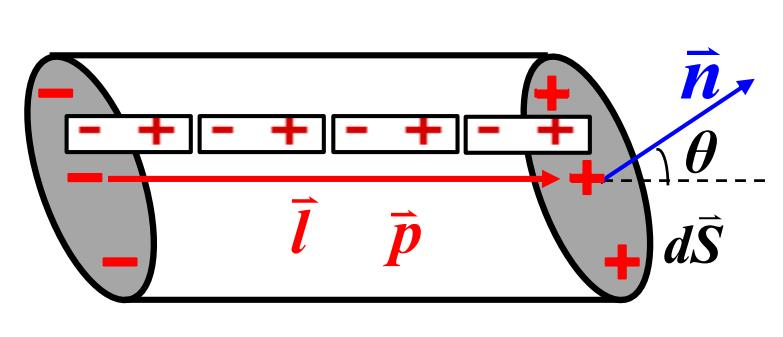
\includegraphics[scale=0.4]{images//chapter_11//figure_11.1.jpg} 
	\caption{有关电极化强度的定理1示意图}\label{figure11.1}
\end{figure}

$$\sigma' =P\cos \theta =\vec{P}\cdot \vec{n_0}=P_n$$

\subsubsection{有关电极化强度的定理2}

二、在电场中,穿过任意闭合曲面的电极化强度通量等于该闭合曲面内\textbf{极化电荷总量}的负值

$$\oint_{S}\vec{P}\cdot d\vec{S}=-\Sigma q' $$

\subsection{电介质中的高斯定理}

$$\oint_{S}\vec{E}\cdot d\vec{S}=\frac{\Sigma q_i+\Sigma q'_i}{\varepsilon_0}$$

其中,$q'$为极化电荷

介质中的高斯定理:
$$\oint_{S}\vec{D}\cdot d\vec{S}=\Sigma q_i$$

其中,$\vec{D}$是电位移矢量,
\begin{equation*}
	\vec{D}=\begin{cases}
		\varepsilon_0 \vec{E}& \text{真空中}\\
		\varepsilon_0 \varepsilon_r \vec{E}& \text{介质中}
	\end{cases}
\end{equation*}

\subsection{电容和电容器}

\subsubsection{电容的定义式}

$$C=\frac{Q}{U_{AB}}$$

\subsubsection{平行板电容器}

$$C=\frac{\varepsilon S}{d}=\frac{\varepsilon_0 \varepsilon_r S}{d}$$

\subsubsection{电容器的连接}

串联:

$$\frac{1}{C_{eq}}=\Sigma \frac{1}{C_i}$$

并联:

$$C_{eq}=\Sigma C_i$$

\subsection{电场的能量}

\subsubsection{电容器的能量}

$$W_e=\frac{Q^2}{2C}=\frac{1}{2}QU=\frac{1}{2}CU^2$$

\subsubsection{电场能量}

电场能量密度:

$$w_e=\frac{1}{2}\varepsilon E^2$$

一定体积内的电场能量

$$W_e=\int_V \frac{1}{2}\varepsilon E^2dV
=\int_V \frac{1}{2}DEdV=\int_V \frac{1}{2\varepsilon} D^2dV$$

\section{恒定磁场}

\subsection{电流密度}

$$\vec{J}=qn\vec{v}$$

电流和电流密度之间的关系:

$$I=\int_{S}\vec{J}\cdot d\vec{S}$$

\subsection{欧姆定律的微分形式}

$$\vec{J}=\sigma \vec{E}$$

$$\vec{E}=\vec{J}\rho $$

其中,$\sigma$为电导率,$\rho$为电阻率

\subsection{磁矩}

对载流线圈(平面),定义磁矩:

$$\vec{p_m}=IS\vec{n}$$

$\vec{n}$:载流线圈的法线方向,与电流构成右手螺旋

\subsection{磁场中的高斯定理与环路定理}

高斯定理:

$$\oint_{S}\vec{B}\cdot d\vec{S}=0$$

安培环路定理:

$$\oint_{L}\vec{B}\cdot d\vec{l}=\mu_0 I$$

\subsection{毕奥萨伐尔定律}

考虑电流元产生的磁场:

$$d\vec{B}=\frac{\mu_0}{4\pi}\frac{Id\vec{l}\times \vec{r}}{r^3}$$

\subsection{毕奥萨伐尔定律的应用}

\subsubsection{载流直导线的磁场}

(见图\ref{figure12.1}所示)

\begin{figure}[h]
	\centering
	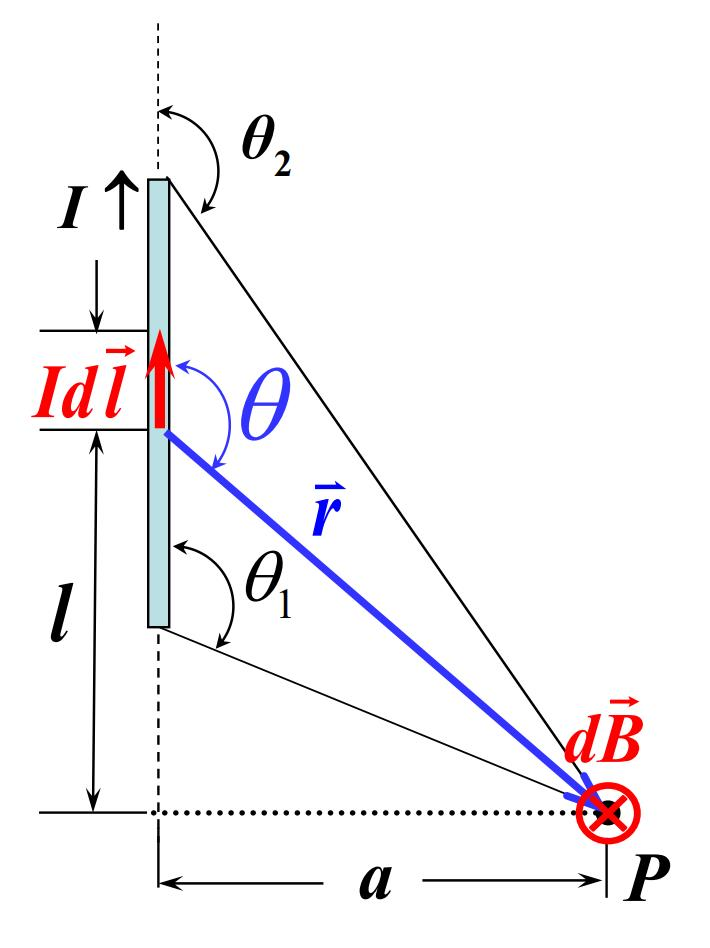
\includegraphics[scale=0.4]{images//chapter_12//figure_12.1.jpg} 
	\caption{载流直导线的磁场}\label{figure12.1}
\end{figure}

$$B=\frac{\mu_0I}{4\pi a}(\cos\theta_1-\cos\theta_2)$$

\textbf{无限长载流直导线}

$$B=\frac{\mu_0I}{2\pi a}$$

\subsubsection{圆形电流轴线上的磁场}

(见图\ref{figure12.2}所示)

\begin{figure}[h]
	\centering
	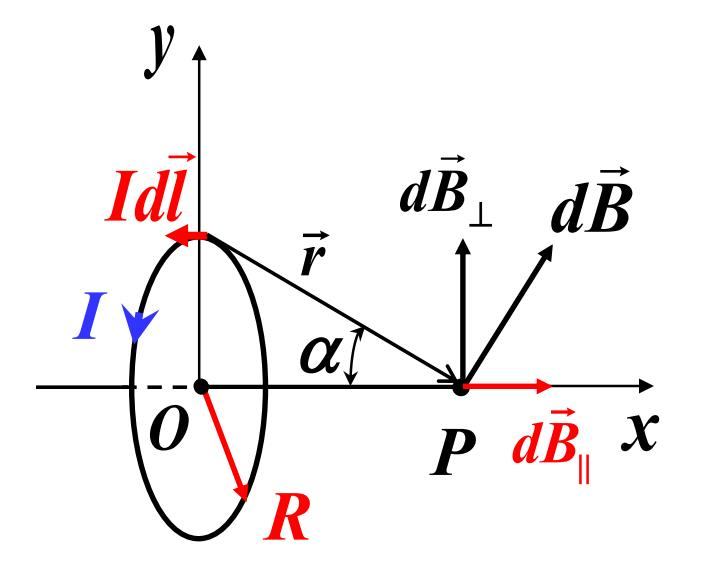
\includegraphics[scale=0.4]{images//chapter_12//figure_12.2.jpg} 
	\caption{圆形电流轴线上的磁场}\label{figure12.2}
\end{figure}

$$\vec{B}=\frac{\mu_0IR^2}{2(R^2+x^2)^{\frac{3}{2}}}\vec{i}$$

\begin{figure}[h]
	\centering
	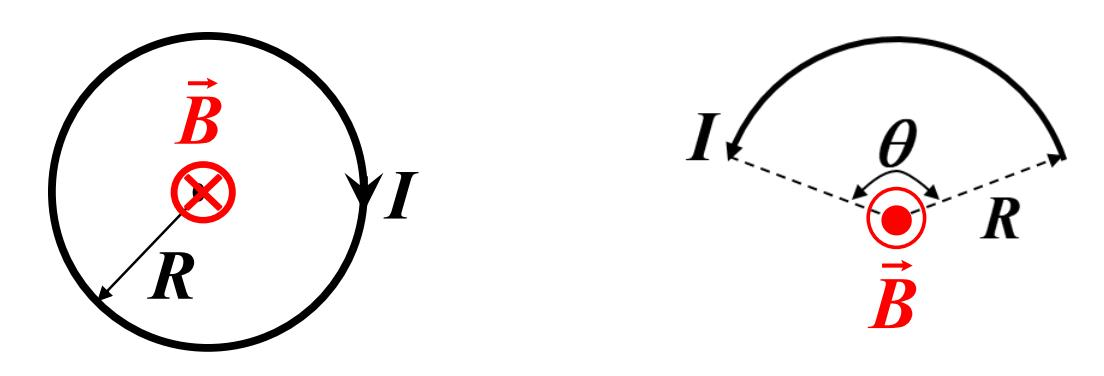
\includegraphics[scale=0.4]{images//chapter_12//figure_12.3.jpg} 
	\caption{圆弧电流在圆心处的磁感应强度}\label{figure12.3}
\end{figure}

\textbf{圆心处的磁感应强度}

$$B=\frac{\mu_0I}{2R}$$

\textbf{圆弧电流在圆心处的磁感应强度}

$$B=\frac{\mu_0I\theta }{4\pi R}$$

\subsubsection{长直螺线管的磁场分布}

(见图\ref{figure12.4}所示)

\begin{figure}[h]
	\centering
	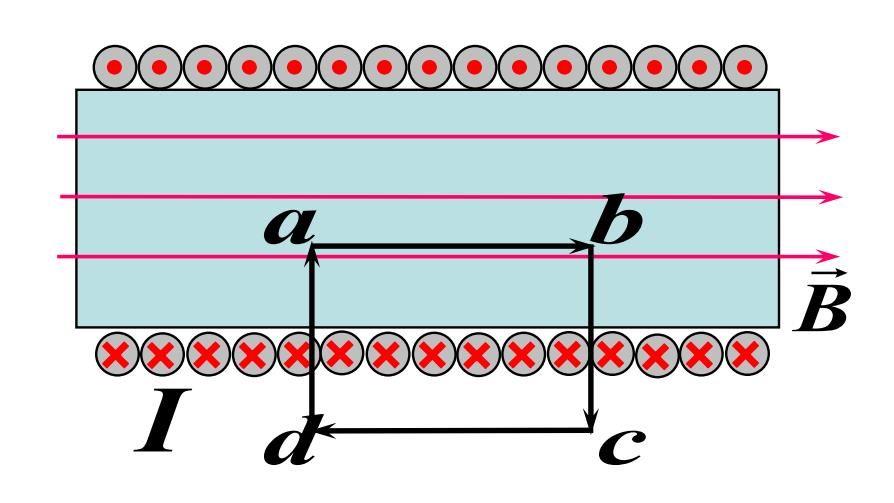
\includegraphics[scale=0.4]{images//chapter_12//figure_12.4.jpg} 
	\caption{长直螺线管的磁场分布}\label{figure12.4}
\end{figure}

\begin{equation*}
	B=\begin{cases}
		\mu_0nI&\text{内}\\
		0&\text{外}\\
	\end{cases}
\end{equation*}

其中,$n$为单位长度导线匝数

\subsection{磁场对载流导线和载流线圈的作用}

\subsubsection{对\textbf{载流导线}的作用:安培定律}

$$d\vec{F}=Id\vec{l}\times\vec{B}$$

\subsubsection{对\textbf{载流线圈}的作用:磁力矩}

$$\vec{M}=\vec{p_m}\times \vec{B}$$

若线圈有$N$匝,则:

$$\vec{M}=N\vec{p_m}\times \vec{B}$$

\subsubsection{磁力做功}

$$W=I\int_{\Phi_{m1}}^{\Phi_{m2}}d\Phi_m=I(\Phi_{m2}-\Phi_{m1})$$

\subsection{磁场对运动电荷的作用}

$$\vec{f}=q\vec{v}\times \vec{B}$$

\subsection{霍尔作用}

\begin{figure}[h]
	\centering
	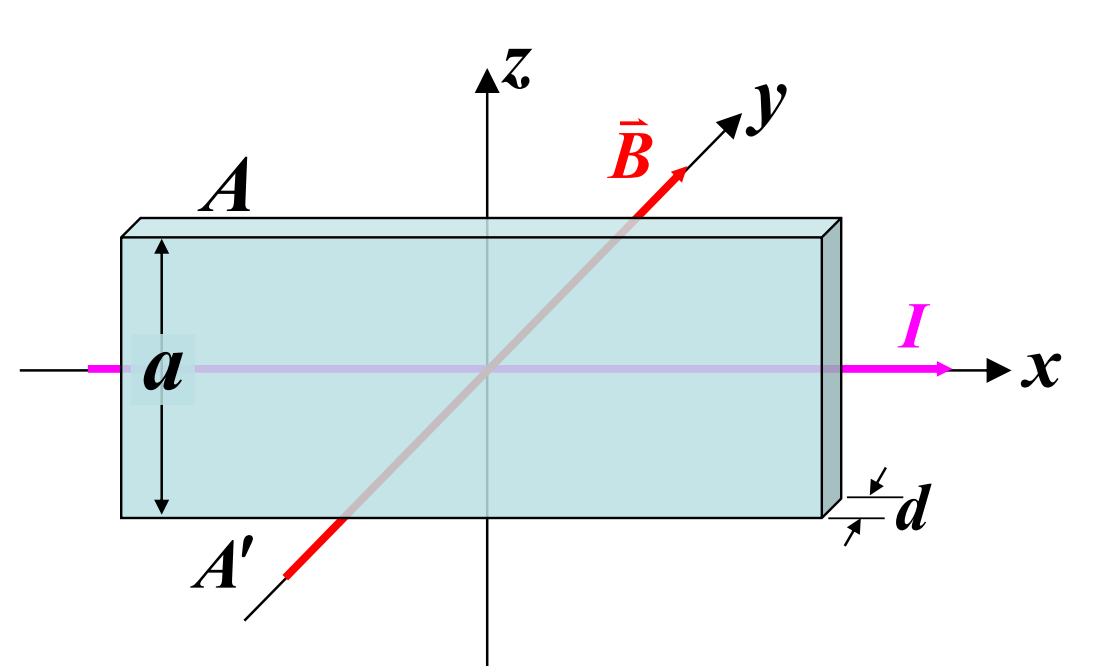
\includegraphics[scale=0.4]{images//chapter_12//figure_12.5.jpg} 
	\caption{霍尔作用}\label{figure12.5}
\end{figure}

霍尔电势差:

$$U_H=R_H\frac{IB}{d}$$

$R_H$为霍尔系数,$R_H=\frac{1}{nq}$,其中$n$为电荷密度。

\section{磁场中的磁介质}

\subsection{相对磁导率}

$$\mu_r=\frac{B}{B_0}$$

$$\begin{cases}
	B>B_0& \text{顺磁质}\mu_r>1\\
	B<B_0& \text{抗磁质}\mu_r<1\\
	B>>B_0& \text{铁磁质}\mu_r>1\\
\end{cases}$$

绝对磁导率:

$$\mu=\mu_0\mu_r$$

\subsection{磁化强度与磁化电流的关系}

磁化强度:

$$\vec{M}=\frac{\Sigma\vec{p_m}}{\Delta V}$$

关系1:

磁化面电流密度等于磁化强度沿介质表面的分量

$$\vec{j_s}=\vec{M}\times \vec{e_n}$$

关系2:

磁化强度对闭合回路$L$的线积分,等于穿过以$L$为周界的任意曲面的磁化电流的代数和

$$\oint_{L}\vec{M}\cdot d\vec{l}=\Sigma I_s$$

\subsection{磁介质中的高斯定理与安培环路定理}

\subsubsection{磁介质中的高斯定理}

$$\oint_{S}\vec{B}\cdot d\vec{S}=0$$

\subsubsection{磁介质中的安培环路定理}

磁介质中:

$$\oint_{L}\vec{B}\cdot d\vec{l}=\mu_0\Sigma (I_{0i}+I_{si})$$

需要包含传导电流与极化电流

令:

$$\vec{H}=\frac{\vec{B}}{\mu_0\mu_r}$$

则有:(此处省略n行推导过程)

$$\oint_{L}\vec{H}\cdot d\vec{l}=\Sigma I_{0i}$$

此时只包括了传导电流。

\subsection{磁极化率}

磁极化率$\chi_m$满足:

$$\chi_m=\mu_r-1$$

(可类比电场中的电极化率)

\section{变化的电磁场}

\subsection{法拉第电磁感应定律}

引入磁链物理量——$\Psi_m=N·\Phi_m$

通过法拉第电磁感应定律计算

——电动势$\varepsilon_i$

$$\varepsilon_i=-\frac{d\Psi_m}{dt}$$

——电流$I$

$$I=\frac{\varepsilon_i}{R}=-\frac{N}{R}\frac{d\Phi_m}{dt}$$

——一段时间内通过线圈的电量$q$

$$q=\int_{t_1}^{t_2}I dt=\int_{t_1}^{t_2}-\frac{N}{R}\frac{d\Phi_m}{dt} dt
=\int_{t_1}^{t_2}-\frac{N}{R}{d\Phi_m}=\frac{N}{R}(\Phi_{m1}-\Phi_{m2})$$

注意是初始磁通减末磁通

\subsection{楞次定律}

高中的\textbf{“增反减同”} 仍可适用,以此来判断感应电动势的方向

\textbf{右手定则:}B穿手心,拇指为切割磁感线速度方向,四指为感应电流方向

\subsection{动生电动势}

非静电力:

$$\vec{f}=-e(\vec{v}\times \vec{B})$$

非静电场强:

$$\vec{E_k}=\frac{f}{-e}=\vec{v}\times \vec{B}$$

导线线元dl的电动势:

$$d\varepsilon = \vec{E}·\vec{dl}=(\vec{v}\times \vec{B})·\vec{dl}$$

整段导线电动势即把$d\varepsilon$ 对$\vec{dl}$积分

\subsection{感生电动势与感生电场}

\textbf{麦克斯韦假设:}

涡旋电场的环路积分=-B对t的偏导数在以环路为边界的面积上的通量

即:

$$\oint_{L} \vec{E_涡}·\vec{dl}=-\oint_{S}\frac{\partial \vec{B}}
{\partial t}·\vec{dS}$$

S的法线方向与边界环路方向满足右手螺旋定则

\subsection{感生电场的运用}

\subsubsection{电子感应加速器}

\begin{figure}[h]
	\centering
	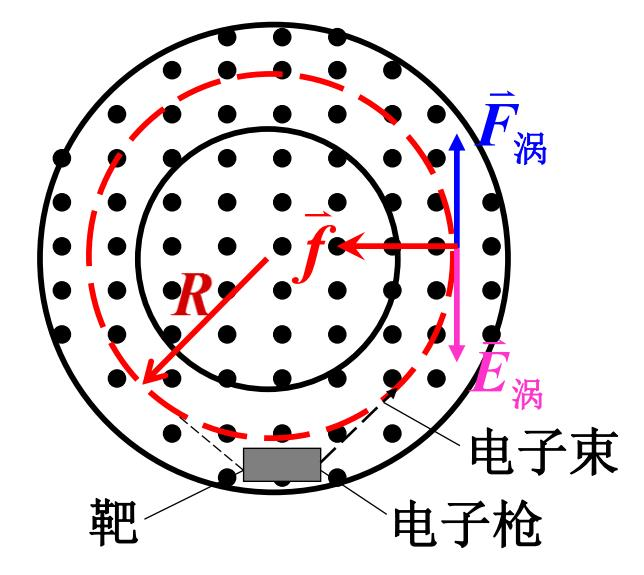
\includegraphics[scale=0.4]{images//chapter_14//figure_14.1.jpg} 
	\caption{电子感应加速器示意图}\label{figure14.1}
\end{figure}


不同于回旋加速器,这里的感应加速器要求半径不变,此时磁场分布应该满足一定条件

由于

$$R=\frac{mv}{eB_R}$$

故,有:

$$eR\frac{dB_R}{dt}=\frac{d(mv)}{dt}$$

而右边式子

$$\frac{d(mv)}{dt}=F_{\text{涡}}=eE_{\text{涡}}$$

又有,

$$E_{\text{涡}}=\frac{1}{2\pi R}\frac{d\Phi_m}{dt}$$

故:
\begin{equation}
\frac{dB_R}{dt}=\frac{1}{2\pi R^2}\frac{d\Phi_m}{dt} \tag{*}
\end{equation}


考虑到电子圆轨道磁通量为$\Phi_m=\pi R^2\bar{B}$,其中,$\bar{B}$为电子
轨道圆内的平均磁感应强度.

将(*)式左右两边对dt积分,得到$B_R=\frac{1}{2}\bar{B}$

电子圆轨道内的磁感应强度若满足该条件,则可以使电子保持在恒定轨道上被加速。

\subsubsection{涡电流}

趋肤效应——涡电流主要分布在导体表层

题型:计算圆柱形涡电流的热功率与热功率密度

\subsection{自感、互感}
\subsubsection{自感系数}

\begin{itemize}
	\item 自感系数定义: $\Psi_m=LI$,
	其中$\Psi_m$ 为磁通链,$L$为自感系数
	
	\item 自感电动势的计算
	
	$$\varepsilon_L=-L\frac{dI}{dt}$$
	
	\item 题型:计算长直螺线管的自感系数
	
	\textbf{基本思路:}求出长直螺线管内部的磁链大小,比去电流$I$,
	得到自感系数(根据定义即可)
	
	注意:这里有些题目需要考虑清楚匝数$N$的选取
\end{itemize}


\subsubsection{互感}

$$\Psi_{21}=M_{21}I_1, \Psi_{12}=M_{12}I_2$$

其中,$M_{21}=M_{12}$ (可以证明得到)

\subsection{自感磁能}

\begin{figure}[h]
	\centering
	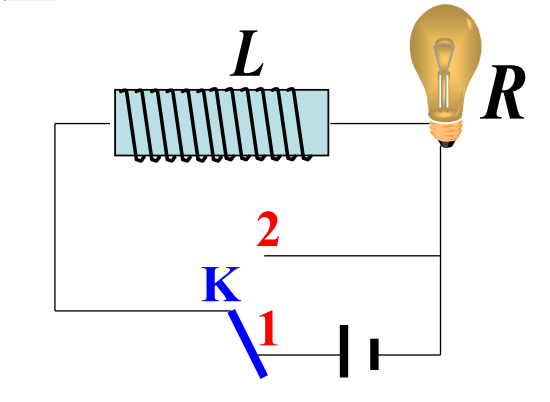
\includegraphics[scale=0.3]{images//chapter_14//figure_14.2.jpg} 
	\caption{电路示意图}\label{figure14.2}
\end{figure}

由全欧姆定律可知:

$$-L\frac{di}{dt}+\varepsilon=iR$$

两边同乘$i$,并且同时对时间积分:

$$\int_{0}^{+\infty}\varepsilon idt=\int_{0}^{I}Lidi+\int_{0}^
{+\infty}i^2Rdt=\frac{1}{2}LI^2+\int_{0}^{+\infty}i^2Rdt$$

上式的物理意义在于:电源对外做功,一部分转化为自感线圈中储存的磁场能,
一部分转化为电阻的焦耳热,而自感线圈中存储的这部分磁能被称为自感磁能,
并且能写出其表达式:

$$W=\frac{1}{2}LI^2$$

到此为止,我们一共有三种计算自感系数的方法:

\begin{enumerate}
	\item 定义法:$L=\frac{\Psi}{I}$
	
	\item 感生电动势:$\varepsilon=-L\frac{di}{dt}$
	
	\item 磁场能量法:$W=\frac{1}{2}LI^2$
\end{enumerate}

\subsubsection{互感磁能}

由上述自感磁能的推导我们可知:电源所做功被转化为两部分:\textbf{1.线圈中产生的焦耳热
2.反抗自感电动势做功},但是当线圈存在互感时,还需要加上\textbf{3.反抗互感
电动势做功},而这一部分能量我们称之为\textbf{互感磁能}

故,系统总磁能为:

$$W=\frac{1}{2}L_1I_1^2+\frac{1}{2}L_2I_2^2+MI_1I_2$$

\subsection{磁场能量}

首先,我们先以螺线管为例,推导出磁场能量密度:

对螺线管而言:$L=\mu n^2V;H=nI;B=\mu nI$

此时磁场能量为:
$$W_m=\frac{1}{2}LI^2=\frac{1}{2}\mu n^2V \left(\frac{B}{\mu n}
\right)^2=\frac{B^2}{2\mu }V$$

可得单位体积内磁场能量,即磁场能量密度$w_E$为:

$$w_m=\frac{B^2}{2\mu }=\frac{1}{2}\mu H^2=\frac{1}{2}BH$$

可以通过一系列理论证明(不要求掌握哈),上述能量密度公式对于任意磁场均成立

且对于任意磁场,其能量为:

$$W=\int_V\frac{B^2}{2\mu }dV=\int_V\frac{1}{2}\mu H^2dV=\int_V \frac{1}{2}BHdV$$

有了能量公式便可以计算出磁能,进而通过“磁场能量法”计算出自感系数。

\subsection{电场能量与磁场能量相比较}

如0下页表\ref{table_1}所示

\begin{table}[h] 
	\centering 
	\renewcommand\arraystretch{1.7}  %%调整行宽为初始值的1.7倍
\begin{tabular}{c c l}
\toprule 
	\textbf{电场能量} & \textbf{磁场能量}  \\
\midrule 
	电容器储能 & 自感线圈储能 \\
	$\frac{1}{2}CU^2=\frac{1}{2}QU=\frac{Q^2}{2C}$ & $\frac{1}{2}LI^2$ \\
	\hline
	电场能量密度 & 磁场能量密度 \\
	$w_e=\frac{1}{2}ED=\frac{1}{2}\varepsilon E^2=\frac{D^2}{2\varepsilon}$	&
	$w_m=\frac{1}{2}BH=\frac{1}{2}\mu H^2=\frac{B^2}{2\mu }$ \\
	\hline
	电场能 & 磁场能(没啥差别,本质就是密度对体积积分~)\\
	$W_E=\int_V w_EdV$ & $W_m=\int_V w_mdV$\\
	\hline
	电场能量法求电容$C$ & 磁场能量法求电感$L$ \\

	\bottomrule 
\end{tabular}
\caption{电场能量与磁场能量相比较}\label{table_1}
\end{table}

\subsection{麦克斯韦电磁场理论(物理学史上的神级理论!)}

麦克斯韦方程组:

\begin{equation*}
	\begin{cases}
		\oint_S \vec{D}·d\vec{S}=\sum q_i=\int_V \rho dV \\
		\oint_L \vec{E}·d\vec{l}=0\\
		\oint_S \vec{B}·d\vec{S}=0\\
		\oint_L \vec{H}·d\vec{l}=\oint_S jd\vec{S}\\
	\end{cases}
\end{equation*}

接下来我们借由前几章已经学过的知识对四个式子
进行物理意义上的解释
\begin{enumerate}
	\item $\oint_S \vec{D}·d\vec{S}=\sum q_i=\int_V \rho dV$
	
	表示电介质中的高斯定理,对任意闭合曲面,电位移矢量在该闭合曲面上的通量
	等于闭合回路内所有自由电荷的代数和(不包括极化电荷)

	注意:该式中电通量流入为负,流出为正。

	\item $\oint_L \vec{E}·d\vec{l}=0$
	
	静电场中的环路定理,体现了电场为无旋场,不是闭合曲线,环路积分得0

	\item $\oint_S \vec{B}·d\vec{S}=0$
	
	\textbf{稳恒磁场}中的高斯定理,体现了磁场为无源场,是闭合曲线,对任意曲面通量得0

	\item $\oint_L \vec{H}·d\vec{l}=\sum I_i=\oint_Sjd\vec{S}$
	
	\textbf{稳恒磁场}中的环路定理,对任意闭合回路,磁场强度的环路积分等于
	穿过由该环路所构成曲面的传导电流代数和
\end{enumerate}

对于变化的电场会产生变化的磁场,即有:

$$\oint_L \vec{E_k}·d\vec{l}=-\oint_S \frac{\partial \vec{B}}
{\partial t}d\vec{S}$$

而对于变化的磁场如何产生变化的电场呢?

麦克斯韦提出了全电流定律,这本是麦克斯韦为解释传统电磁理论在
电容中的不适用性而引入位移电流后得出的式子,具体推导过程了解即可。

\subsubsection{全电流定律}

\textbf{全电流定律表述如下:}

$$\oint_L \vec{H}·d\vec{l}=\oint_S (j+\frac{\partial\vec{D}}{\partial t})d\vec{S}$$

\textbf{物理意义:变化磁场} 中的环路定理,对任意闭合回路,磁场强度的环路积分等于
穿过由该环路所构成曲面的传导电流与\textbf{位移电流}的代数和,其中$\frac{
	\partial D}{\partial t}$为\textbf{位移电流密度}

\textbf{位移电流的定义:}单位时间内极板上电荷的增加(减少)等于流入(或流出)极板的电流

$$I=\frac{dQ}{dt}=\frac{d\Phi_d}{dt}=\int_S\frac{\partial \vec{D}}{
\partial t}·d\vec{S}$$

从定义式中可看出,位移电流可认为是两极板间电位移通量随时间的变化率。

\textbf{位移电流的方向:}

\begin{figure}[h]
	\centering
	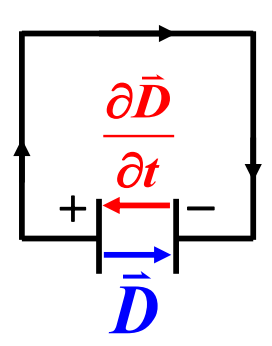
\includegraphics[scale=0.3]{images//chapter_14//figure_14.3.jpg} 
	\caption{位移电流方向示意图}\label{figure14.3}
\end{figure}

当电容器放电时,$q\downarrow\rightarrow\sigma\downarrow D\downarrow$

(其中借用了电位移矢量的边界条件:D在边界处的法向分量为该边界处电荷面密度)

故,$\frac{\partial\vec{D}}{\partial t}$与$\vec{D}$反向

\subsection{各向同性介质的物质方程}

当有介质存在时,$\vec{E}$和$\vec{B}$的存在与介质的特性有关,故需要补充
物质方程以使麦克斯韦方程组更加完备,现补充物质方程如下:

\begin{equation*}
	\begin{cases}
		\vec{D}=\varepsilon_0\varepsilon_r \vec{E}=\varepsilon\vec{E}\\
		\vec{B}=\mu_0\mu_r\vec{H}=\mu \vec{H}\\
		\vec{j}=\sigma\vec{E}\text{欧姆定律的微分形式,其中}\sigma \text{为
		电导率,而非面密度}\\
	\end{cases}
\end{equation*}

\subsection{电磁波}

\subsubsection{电磁波波动方程}

由麦克斯韦理论,在自由空间中的电场和磁场满足:

$$\oint \vec{E_k}\cdot d\vec{l}=-\int \frac{\partial \vec{B}}{\partial t}\cdot d\vec{S}$$

$$\oint \vec{H}\cdot d\vec{l}=\int \frac{\partial \vec{D}}{\partial t}\cdot d\vec{S}$$

\subsubsection{平面电磁波基本性质}

\begin{figure}[h]
	\centering
	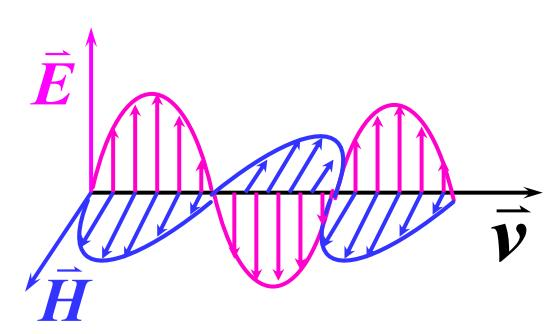
\includegraphics[scale=0.3]{images//chapter_14//figure_14.4.jpg} 
	\caption{平面电磁波示意图}\label{figure14.4}
\end{figure}

\begin{enumerate}
	\item 电磁波是横波,$\vec{E},\vec{H},\vec{v}$相互垂直,呈右螺关系
	\item $\vec{E}$和$\vec{H}$同相位、同频率
	\item 电磁场中任意一点都满足$$\sqrt{\varepsilon}E=\sqrt{\mu}H$$
	\item 电磁波传播速度$$v=\frac{1}{\sqrt{\varepsilon\mu}}$$
\end{enumerate}

\subsubsection{电磁波能量密度}

$$w=w_e+w_m=\frac{1}{2}(\varepsilon E^2+\mu H^2)=\varepsilon E^2=\mu H^2$$

\subsubsection{电磁波能量}

$$W=\int_V wdV=\int_V \varepsilon E^2dV=\int_V \mu H^2dV$$

\subsubsection{电磁波的能流密度}

坡印廷矢量——

$$\vec{S}=\vec{E}\times \vec{H}$$

\section{量子力学}

\subsection{早期量子论}

\subsubsection{黑体}

\begin{enumerate}
	\item 黑体是能全部吸收各种入射电磁波的物体,它不是黑色的!(震声!)
	\item 单色辐射本领$M_\lambda(T)$
	\textbf{定义:}
	\textbf{单位时间内},从物体表面\textbf{单位面积}上发射的波长在$\lambda$附近\textbf{单位波长}间隔内的辐射能。
	\item 辐射出射度(辐出度)$M(T)$
	\textbf{定义:}
	\textbf{单位时间内},从物体表面\textbf{单位面积}发射的各种波长的总辐射能
	
	计算公式:$$M(T)=\int_0^\infty M_\lambda(T)d\lambda$$
	$M(T)$在量值上等于单位表面积的辐射功率

	如果已知太阳的半径,再通过后面提到的斯特藩-玻尔兹曼定律
	求出$M(T)$,即可求出太阳的辐射功率——
	$$P=4\pi R^2\times M(T)=4\pi R^2\times \sigma T^4$$

	\item 上述的$T$,又可以用维恩位移定律$\lambda_m T=b$求得。
    \textbf{——这个思路已经在历年考题中出现了5,6次,务必记牢。}

\end{enumerate}

\subsubsection{斯特藩-玻尔兹曼定律}
\begin{enumerate}
	\item 黑体辐射的总辐射本领(辐射出射度)$$M(T)=\int_0^\infty M_\lambda(T)d\lambda$$
	\item 定律公式:$$M(T)=\sigma T^4$$
	\item 斯特藩-玻尔兹曼常量$\sigma =
	5.67\times 10^{-8}W\cdot m^{-2}\cdot K^{-4}$(可以不用记)
\end{enumerate}

\subsubsection{维恩位移定律}
\begin{enumerate}
	\item 定律公式:$$\lambda_m T=b$$
	\item 维恩常数 $b=2.898\times 10^{-3}m\cdot K$
	\item 黑体温度升高时,单色辐出度最大值向短波方向移动
\end{enumerate}

\subsection{光电效应}

\subsubsection{光电效应伏安特性曲线}

(如图\ref{figure15.1}所示)

\begin{figure}[h]
	\centering
	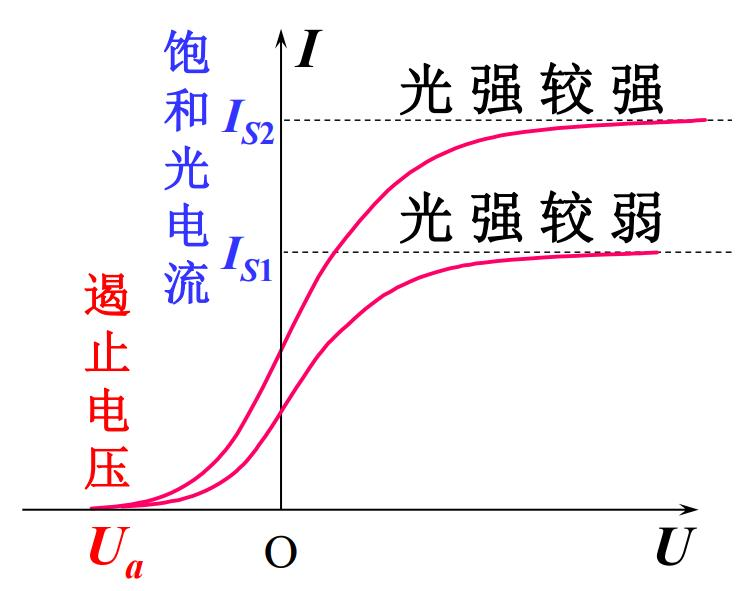
\includegraphics[scale=0.3]{images//chapter_15//figure_15.1.jpg} 
	\caption{光电效应伏安特性曲线}\label{figure15.1}
\end{figure}

\subsubsection{光电效应的规律与易错点}
\begin{enumerate}
	\item 饱和光电流与入射光强度成正比
	\item 最大初动能与入射光频率有关,与入射光强度无关
	\item 截止电压与入射光频率有关,与入射光强度无关
	\item 最大初动能与频率成线性关系
\end{enumerate}

\subsubsection{定量分析}
\begin{enumerate}
	\item 爱因斯坦光电效应方程
	$$h\upsilon = \frac{1}{2}mv^2+W$$
    其中,
    $\upsilon$为入射光频率,
    $\frac{1}{2}mv^2$为出射电子动能,
    $W$为逸出功,每个金属的逸出功都不一样,
    $h=6.63\times 10^{-34}J\cdot s$
	\item 引入截止电压$U_a$
    $$eU_a=\frac{1}{2}mv^2$$
	\item 红限频率$\upsilon_0$
    即为:出射电子动能为0时的频率,此时为临界状态
    $$h\upsilon_0 =W$$
	\item 爱因斯坦的光电效应方程与光量子理论体现了\textbf{光的粒子性}。
\end{enumerate}

\subsection{光的波粒二象性}

\subsubsection{光子能量}

$$\varepsilon =h\upsilon$$

$$\varepsilon=mc^2$$

\subsubsection{光子质量}

$$m=\frac{\varepsilon}{c^2}=\frac{h\upsilon}{c^2}$$

\subsubsection{光子动量}

$$p=mc=\frac{\varepsilon}{c}=\frac{h\upsilon}{c}=\frac{h}{\lambda}$$

\subsection{康普顿效应}

\subsubsection{效应内容:}

X射线通过物质散射时,发现散射光中除了有原波长的X光以外,
还产生了波长增长的X光,这种现象称为康普顿效应.

\subsubsection{试验规律(了解即可)}
\begin{enumerate}
	\item 散射X射线波长有两个峰值,即:散射光中有波长不变的X射线,也有波长变长的X射线
	\item 波长的改变量与散射角有关
	\item 不同元素的散射物质,在同一散射角下,波长改变量$\Delta \lambda$相同
	\item 波长为$\lambda$的散射光强度随散射物质原子序数增加而减小
\end{enumerate}

\subsubsection{定量分析}

\begin{figure}[h]
	\centering
	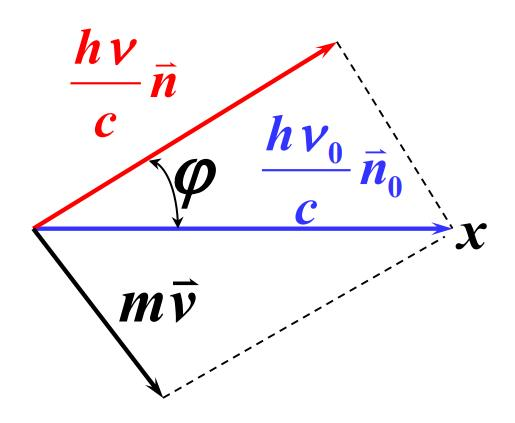
\includegraphics[scale=0.3]{images//chapter_15//figure_15.2.jpg} 
	\caption{动量守恒示意图}\label{figure15.2}
\end{figure}

\begin{enumerate}
	\item 能量守恒——
	$$mc^2+h\upsilon =m_0c^2+h\upsilon_0$$
	\item 动量守恒——
	$$\frac{h\upsilon_0}{c}\vec{n}=m\vec{v}+\frac{h\upsilon}{c}\vec{n}$$
	\item 康普顿散射公式——
	$$\Delta \lambda=\lambda-\lambda_0=\frac{2h}{m_0c}sin^2\frac{\varphi}{2}$$
	\item 康普顿效应体现了光的粒子性。
\end{enumerate}

\subsection{玻尔的氢原子理论}

\subsubsection{巴耳末系公式}

$$\frac{1}{\lambda}=R(\frac{1}{4}-\frac{1}{n^2})$$

其中,$n=3,4,5,\cdots$

\subsubsection{三个假设}
\begin{enumerate}
	\item 定态假设
	原子其电子只能在确定轨道上绕核作圆周运动
	\item 频率假设
	原子从一较大能量$E_n$的定态向另一较低能
	量$E_k$的定态跃迁时,辐射一个光子,光子频率满足:
	$$h\upsilon=E_n-E_k$$
	\item 轨道角动量量子化假设
	原子中电子绕核运动的轨道角动量是量子化的;
	\item $L=n\hbar $
	其中,$n$为量子数,
	$\hbar$为约化普朗克常数。
\end{enumerate}


\subsubsection{三个量子化}
\begin{enumerate}
	\item 角动量量子化(同上)
	\item 轨道半径量子化
	$$r_n=0.53n^2\overset{\circ }{A}$$
	其中,$n=1,2,3,\cdots$
	\item 能量量子化
    $$E_n=\frac{-13.58}{n^2}eV$$
    其中,$n=1,2,3,\cdots$
\end{enumerate}

\subsubsection{巴耳末系的最短波长与最长波长}

最长波长$\lambda_{\max}$是由$n=3$→$n=2$跃迁产生的光波

$$\frac{1}{\lambda_{\max}}=R(\frac{1}{2^2}-\frac{1}{3^2})$$

最短波长$\lambda_{\min}$是由$n=\infty$→$n=2$跃迁产生的光波

$$\frac{1}{\lambda_{\min}}=R(\frac{1}{2^2}-\frac{1}{\infty^2})=R(\frac{1}{2^2})$$

\textbf{期末常考}:最短波长与最长波长的比值?最长波长与第二长波长比值?

注:跃迁\textbf{到}$n=2$的光波属于巴耳末系

\subsection{德布罗意波}

\subsubsection{德布罗意关系式}
\begin{enumerate}
	\item 能量公式(同上)
    $$E=mc^2=h\upsilon$$
	\item 动量公式(同上)
    $$p=mv=\frac{h}{\lambda}$$
	\item 自由粒子速度较小时
    $$E_k=\frac{p^2}{2m}$$
    $$\lambda=\frac{h}{p}=\frac{h}{\sqrt{2mE_k}}=\frac{h}{\sqrt{2meU}}$$
\end{enumerate}

\subsubsection{相关实验汇总}
\begin{enumerate}
	\item 戴维孙-革末进行了电子衍射实验,证明了电子的波动性
	\item $G.M.$进汤姆逊进行了电子衍射实验,证明了电子的波动性
	\item 斯特恩实验证明中性原子和分子也具有波动性
\end{enumerate}

\subsection{不确定关系}

\subsubsection{动量与位置的不确定关系}

$$\Delta x\Delta p\ge \frac{\hbar}{2}$$

动量与位置不能同时确定

\subsubsection{能量与时间的不确定关系}

$$\Delta E\Delta t\ge \frac{\hbar}{2}$$

能量与时间不能同时确定

\subsection{薛定谔方程}

\subsubsection{定态波函数}

$$-\frac{\hbar^2}{2m}\bigtriangledown ^2\Psi=(E-U)\Psi$$

其中,
$\bigtriangledown ^2$是拉普拉斯算符,在一维波函数里满足:
$$\bigtriangledown ^2\Psi=\frac{\partial \Psi^2}{\partial^2 x}$$
$E$为能量,
$U$为势能函数

注:\begin{enumerate}
	\item 波函数为复数函数,无确定的物理意义
	\item 波函数模的平方表征概率密度函数
	$$w=|\Psi (x)|^2$$
	\item 归一化条件:(一维情况下)
	$$\int_{-\infty}^{+\infty} wdx=1$$
	\item 波函数的标准条件:单值、有限、连续(考过一次);
	\item 等价条件:
	$\Psi  = C\Psi$,
	其中$C$为常数,使得$\Psi$能够满足归一化条件;
\end{enumerate}

\subsubsection{波函数的计算}

(常考题型,建议记结论)

假定波函数

$$\Psi_n(x)=Asin(\frac{n\pi}{a}x)$$

由概率密度函数的归一化条件

$$\int_{-\infty}^{+\infty} |\Psi(x)|^2dx=\int_{-\infty}^{+\infty} A^2sin^2(\frac{n\pi}{a}x)dx=1$$
    
由积分结果可以得到$$A=\sqrt{\frac{2}{a}}\text{(记!)}$$

求:$0\rightarrow a/2$区间内,粒子出现概率

计算方法:

$$\int_{0}^{a/2} \frac{2}{a}sin^2(\frac{n\pi}{a}x)dx=\frac{1}{2}$$

小规律:

$0\rightarrow ma$区间内,粒子出现概率为$m$,和$n$无关,和$a$也无关

推论:

$ma\rightarrow qa$区间内,粒子出现概率为$q-m$,和$n$无关,和$a$也无关

\subsubsection{隧穿效应}

势垒越宽透过的概率越小

$(U_0-E)$越大透过的概率越小

隧道效应是不确定原理的体现,其本质是微观粒子的波粒二象性

\subsubsection{一维线性谐振子}

谐振子能量
    
$$E_n=(n+\frac{1}{2})\hbar \omega$$

其中,$n=0,1,2,\cdots$

\subsection{氢原子的量子理论}

\subsubsection{三个量子数}

主量子数$n$:$n=1,2,3,\cdots$

角量子数$l$:$l=0,1,2,\cdots,(n-1)$,角动量$L=\sqrt{l(l+1)}\hbar$

角动量空间取向量子化-磁量子数$m_l$

$m_l=0,\pm 1,\pm 2,\cdots,\pm l$

\subsection{多电子原子中电子分布规律}

(参见高中化学-物构部分)

斯特恩—盖拉赫实验证明了角动量的空间取向是量子化的

\subsubsection{电子的轨道磁矩}

(了解即可)

$$\vec{\mu}=-\frac{e}{2m}\vec{L}$$

\subsubsection{电子自旋}

电子自旋角动量——

$$S=\sqrt{s(s+1)}\hbar$$

其中,$s$为自旋量子数,$s=\frac{1}{2}$

自旋磁量子数$m_s=\pm \frac{1}{2}$

\subsubsection{电子排布规律}

用四个量子数表征$(n,l,m_l,m_s)$

例: 电子在3d轨道上:

$n=3,l=2,m_l=0,\pm 1,\pm 2, m_s=\pm \frac{1}{2}$

注:
\begin{enumerate}
	\item $l$的记号
	\begin{tabular}{c|c|c|c|c|c|c|c|c|c}
	$l$& 0 & 1 & 2 & 3 & 4 & 5 & 6 & 7 & 8 \\
	\hline
	记号& s &  p &  d & f & g & h & i & k & l\\
	\end{tabular}
	\item 磁量子数$m_l=0,\pm 1,\pm 2,\cdots,\pm l$
	\item 自旋量子数$m_s=\pm \frac{1}{2}$
\end{enumerate}

\subsection{泡利不相容原理}

\begin{enumerate}
	\item 当$n$给定时,$l$的可能取值有$n$个
	\item 当$l$给定时,$m_l$的可能取值有$2l+1$个
	\item 当$n,l,m_l$给定时,$m_s=\pm \frac{1}{2}$共2个
	\item 给定主量子数为$n$的壳层上,可能有的最多电子数为$2n^2$
\end{enumerate}

\section{激光}

\begin{enumerate}
	\item 受激辐射光放大是激光产生的\textbf{基本机制}
	\item 粒子数反转是产生激光的\textbf{最关键因素}
\end{enumerate}

\subsection*{激光的特性}

\begin{enumerate}
	\item 单色性好
	\item 相干性好
	\item 方向性好
	\item 亮度高,能量集中
\end{enumerate}

\subsection*{激光产生的条件}

受激辐射,粒子数反转,三能极系统,谐振腔\textbf{(没有自发辐射)}

\end{document}